\chapter{Methodology}
\label{ch_methods}

We designed a general process for evaluating the state of the practice of domain-specific SC software, that we instantiate for a specific scientific domain.

Our method involves four steps:
\begin{enumerate}
\item choosing a software domain (Section \ref{sec_domain_selection});
\item collecting and filtering software packages (Section \ref{sec_software_selection});
\item grading the selected software (Section \ref{sec_grading_software});
\item interviewing development teams for further information (Section \ref{sec_interview_methods}).
\end{enumerate}

\noindent Section \ref{sec_applying_method} presents an example of how we applied the method on the MI domain.

\section{Domain Selection}
\label{sec_domain_selection}
Our methods are generic for any SC software, but they need to be applied to a specific domain. When choosing a candidate domain, we prefer one with a large number of active OSS. The reason is that we aim to finalize a list of 30 software packages \cite{SmithEtAl2021} after the screening step. For example, we remove the ones without recent updates or specific functions. Besides, we prefer OSS projects because our grading method requires access to the code. In addition, we prefer a domain with an active community developing and using the software. As a result, it is easier to invite enough developers for interviews.

We prefer 30 software packages providing similar functions or falling into different sub-groups depending on our research purpose. So the domain needs to have enough candidates in one sub-group or enough sub-groups to cross-compare.

We also prefer domains in which our team has expertise. We invite domain experts to join and support our projects. They help us in many aspects, such as vetting the software list and interview questions.

\section{Software Product Selection}
\label{sec_software_selection}

The process of selecting software packages contains two steps: i) identify software candidates in the chosen domain, ii) filter the list according to our needs \cite{SmithEtAl2021}.

\subsection{Identify Software Candidates}
\label{sec_identify_software_candidates}
We start with finding candidate software in publications of the domain. Then, we search various websites, such as \hyperlink{https://github.com/}{GitHub}, \hyperlink{https://swmath.org/}{swMATH} and the Google search results for software recommendation articles. We should also include the ones suggested by the domain experts \cite{SmithEtAl2021}.

\subsection{Filter the Software List}
\label{sec_filter_software_list}
The goal is to build a software list with a length of about 30 \cite{SmithEtAl2021}.

The only ``mandatory'' requirement is that the software must be OSS, as defined in Section \ref{sec_open_source_software}. We need this because evaluating some software qualities requires the source code.

The other filters are optional, and we consider them according to the number of software candidates and the objectives of the research project. We apply them in the following priority order:

\begin{enumerate}
\item The functions and purpose of the software. An SC domain often contains software with various functions and purposes. For example, some MI software packages are Tool Kit for developers to use, and some others offer Visualization function to end-users. We have two options:
\begin{itemize}
\item selecting a set of software with the same major function. In this case, we can use the identical process to assess all packages, e.g., same input to measure \textit{Robustness}. Also, when we give impression scores to qualities such as \textit{Installability} and \textit{Usability}, the results are more comparable. Thus, it is more feasible to collect the results and rank the software.
\item selecting software from a set of different sub-groups. For example, we can choose 10 MI software from each of the three sub-groups: Visualization, Tool Kit, and PACS. The downside: we may need different processes to measure each sub-group; it may be less accurate to mix all three sub-groups and rank them together. The benefit: we can cross-compare the development processes between the sub-groups.
\end{itemize}

\item The version control tool. The empirical measurement tools listed in Section \ref{sec_empirical_measurements} only work on projects using \hyperlink{https://git-scm.com/}{Git}, so we prefer software with Git. Some manual steps in empirical measurement depend on a few metrics of GitHub, which makes projects held on GitHub more favored \cite{SmithEtAl2021}.

\item The age of the software. Some of the OSS projects may experience a lack of recent maintenance. So we eliminate packages without recent updates, unless they are still popular and highly recommended by the domain users \cite{SmithEtAl2021}. We consider a software project as ``alive" if it has any update within the last 18 months; otherwise, we mark it as ``dead".
\end{enumerate}

The order of filters 2 and 3 is flexible. We adjust it according to the number of software packages affected by the filters, and the number of ones remaining on the list.

\subsection{Vet the Software List}
\label{sec_vet_software_list}
Before showing our filtered list to the domain experts, we ask them to list their top 10 software in the domain. Then, we cross-compare the two lists and discuss the commonality and variability.  In addition, we ask them to vet our filtered list. They provide views on whether the list is reasonable. We also use their opinions for a filtering process. For example, if a software package is not OSS and has had no updates for a long time, but the domain experts identify it as a valuable product, we still consider it in our final list.

\section{Grading Software}
\label{sec_grading_software}

We grade the selected software using a template (Section \ref{sec_grading_template}) and a specific empirical method (Section \ref{sec_empirical_measurements}). Some technical details for the measurements are in Section \ref{sec_technical_details}.

\subsection{Grading Template}
\label{sec_grading_template}
The full grading template can be found in Appendix \ref{ap_grading_template}. The template contains 103 questions that we use for grading software products. Figure \ref{fg_grading_template_example} shows an example of this grading template.

\begin{figure}[h]
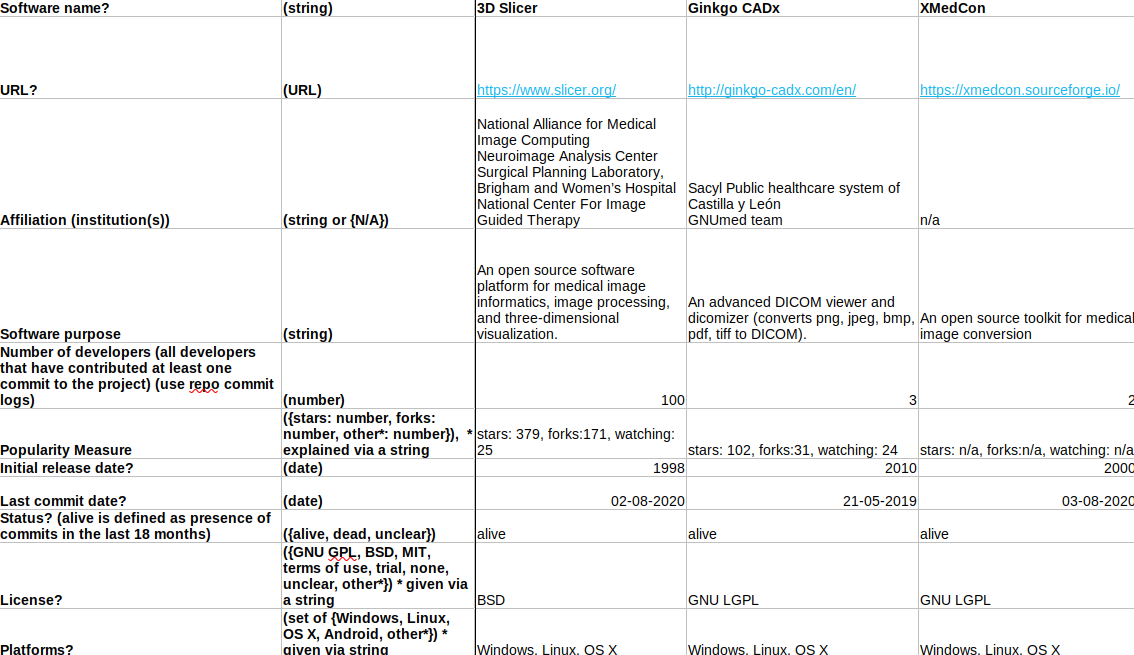
\includegraphics[scale=0.42]{figures/template.png}
\caption{Grading template example}
\label{fg_grading_template_example}
\end{figure}

We use the first section of the template to collect general information, such as the name, purpose, platform, programming language, publications about the software, the first release and the most recent change date, website, source code repository of the product, etc. Information in this section helps us understand the projects better and may be helpful for further analysis, but it does not directly affect the grading scores.

We designed the following nine sections in the template for the nine software qualities mentioned in Section \ref{sec_software_quality}. For each quality, we ask several questions and the typical answers are among the collection of ``yes'', ``no'', ``n/a'', ``unclear'', a number, a string, a date, a set of strings, etc. Each quality needs an overall score between 1 and 10 based on all the previous questions. For some qualities, we perform surface measurements, which allow us to measure all packages with reasonable efforts. The surface measurements reveal some traits of a underlying quality, but may not fully represent it.

\begin{itemize}
\item \textbf{Installability} We check the existence and quality of installation instructions. The user experience is also an important factor, such as the ease to follow the instructions, number of steps, automation tools, and the prerequisite steps for the installation. If any problem interrupts the process of installation or uninstallation, we give a lower score to this quality. We also record the Operating System (OS) for the installation test and whether we can verify the installation.

\item \textbf{Correctness \& Verifiability} For \textit{correctness}, we check the projects to identify the techniques to ensure this quality, such as literate programming, automated testing, symbolic execution, model checking, unit tests, etc. We also examine whether the projects use continuous integration and continuous delivery (CI/CD). For \textit{verifiability}, we go through the documents of the projects to check the requirements specifications, theory manuals, and getting started tutorials. If a getting started tutorial exists and provides expected results, we follow it and check if the outputs match.

\item \textbf{Surface Reliability} We check whether the software breaks during the installations and tutorials, whether there are descriptive error messages, and if we can recover the process after an error.

\item \textbf{Surface Robustness} We check how the software handles unexpected/unanticipated input. For example, we prepare broken image files for software packages with the function to load image files. We use a text file (.txt) with a modified extension name (.dcm) as an unexpected/unanticipated input. We load a few correct input files to ensure the function is working correctly before testing with the unexpected/unanticipated ones.

\item \textbf{Surface Usability} We examine the documentation of the projects, and we consider software with a getting started tutorial and a user manual easier to use. Meanwhile, we check if users have any channels to get support. We also record our impressions and user experiences when testing the software. Easy-to-use graphical user interfaces give us a better experience, which leads to better scores.

\item \textbf{Maintainability} We search the projects' documents and identify the process of contributing and reviewing code. We believe that the artifacts of a project - including source code, documents, building scripts, etc. - can significantly affect its  \textit{maintainability}. Thus we check each project for its artifacts, such as API documentation, bug tracker, release notes, test cases, build files, version control, etc. We also check the tools supporting issue tracking and version control, the percentages of closed issues, and the proportion of comment lines in code.

\item \textbf{Reusability} We count the total number of code files for each project. Projects with a large number of components provide more choices to reuse. Furthermore, well-modularized code, which tends to have smaller parts in separated files, is typically easier to reuse. Thus, we consider the projects with more code files to be more reusable. We use \textit{GitStats} as a tool to count the number of text-based files for all projects, and consider the projects with more text-based files to also have more code files. We also decide that the projects with API documentation can deliver better \textit{Reusability}.

\item \textbf{Surface Understandability} We randomly examine 10 code files. We check the code’s style within each file, such as whether the identifiers, parameters, indentation, and formatting are consistent, whether the constants (other than 0 and 1) are hardcoded, and whether the developers modularized the code. We also check the descriptive information for the code, such as documents mentioning the coding standard, the comments in the code, and the descriptions or links for algorithms in the code. 

\item \textbf{Visibility/Transparency} To measure this quality, we check the existing documents to find out whether the software development process and current status of a project are visible and transparent. We examine the development process, current status, development environment, and release notes for each project. If any information is missing or poorly conveyed, the \textit{visibility/transparency} will be lower.
\end{itemize}

For some qualities, the empirical measurements also affect the score. We use tools to extract information from the source code repositories. For projects held on GitHub, we manually collect additional metrics, such as the stars of the GitHub repository, and the numbers of open and closed pull requests. Section \ref{sec_empirical_measurements} presents more details about the empirical measurements.

\subsection{Empirical Measurements}
\label{sec_empirical_measurements}

We use two command-line tools for the empirical measurements. One is \textit{GitStats} that generates statistics for git repositories and displays outputs in the form of web pages \cite{Gieniusz2019}; the other one is Sloc Cloc and Code (as known as \textit{scc}) \cite{Boyter2021}, aiming to count the lines of code, comments, etc.

Both tools measure the number of text-based files in a git repository and lines of text in these files. Based on our experience, most text-based files in a repository contain programming source code, and developers use them to compile and build software products. A minority of these files are instructions and other documents. So we roughly regard the lines of text in text-based files as lines of programming code. The two tools usually generate similar but not identical results. From our understanding, this minor difference is due to the different techniques to detect if a file is text-based or binary.

Additionally, we manually collect information for projects held on GitHub, such as the numbers of stars, forks, people watching this repository, open pull requests, closed pull requests, and the number of months a repository has been on GitHub. A git repository can have a creation date much earlier than the first day on GitHub. For example, the developers created the git repository of \textit{3D Slicer} in 2002, but did not upload a copy of it to GitHub until 2020. We get the creation date of the GitHub copy by using API \textit{https://api.github.com/repos/{:owner}/{:repository}} (e.g., \hyperlink{https://api.github.com/repos/slicer/slicer}{https://api.github.com/repos/slicer/slicer}). In the response, the value of ``created\_at" is what we want. The number of months a repository has been on GitHub helps us understand the average change of metrics over time, e.g., the average new stars per month. 

These empirical measurements help us from two aspects. Firstly, they help us with getting a project overview faster and more accurately. For example, the number of commits over the last 12 months shows how active this project has been, and the number of stars and forks may reveal its popularity. Secondly, the results may affect our decisions regarding the grading scores for some software qualities. For example, if the percentage of comment lines is low, we double-check the \textit{understandability} of the code; if the ratio of open versus closed pull requests is high, we pay more attention to the \textit{maintainability}.

\subsection{Technical Details}
\label{sec_technical_details}
To test the software on a ``clean'' system, we create a new virtual machine (VM) for each software and only install the necessary dependencies before measuring. We make all 30 VMs on the same computer, one at a time, and destroy them after measuring.

We spend about two hours grading each package, unless we find technical issues and need more time to resolve them. In most of the situation, we finish all the measurements for one software on the same day.

\section{Interview Methods}
\label{sec_interview_methods}

This section introduces our interview questions (Section \ref{sec_interview_questions}), method of selecting interviewees (Section \ref{sec_interviewee_selection}), and interview process (Section \ref{sec_interview_process}).

\subsection{Interview Questions}
\label{sec_interview_questions}
We designed a list of 20 questions to guide our interviews, which can be found in Section \ref{ch_interview} and Appendix \ref{ap_interview}.

Some questions are about the background of the software, the development teams, the interviewees, and how they organize the projects. We also ask about their understandings of the users. Some questions focus on the current and past difficulties, and the solutions the team has found or will try. We also discuss the importance and current situations of documentation. A few questions are about specific software qualities, such as \textit{maintainability}, \textit{understandability}, \textit{usability}, and \textit{reproducibility}.

The interviews are semi-structured based on the question list; we ask follow-up questions when necessary. Based on our experience, the interviewees usually bring up some exciting ideas that we did not expect, and it is worth expanding on these topics.

\subsection{Interviewee Selection}
\label{sec_interviewee_selection}
For a software list with a length of roughly 30, we aim to interview about ten development teams. Interviewing multiple individuals from each team gives us more comprehensive information, but a single engineer well-knowing the project is also sufficient.

Ideally, we select projects after the grading measurements and prefer the ones with higher overall scores. However, if we do not find enough participants, we reach all teams on the list. As mentioned in Section  \ref{sec_apply_to_mi_interviews}, when we applied this process to the MI domain, we eventually contacted all teams.

We try to find the contacts of the teams on the projects' websites, such as the official web pages, repositories, publications, and bio pages of the teams' institutions. Then, we send at most two emails to one contact asking for its participation before receiving any replies. We operate the invitation according to our ethics approval, such as the one in Appendix \ref{ap_ethics}. For example, we ask for participants' consent before interviewing them, recording the conversation, or including it in our report.

\subsection{Interview Process}
\label{sec_interview_process}
Before contacting any interviewee candidate, we need to receive ethics clearance from the McMaster University Research Ethics Board. Since the members of the development teams are usually around the world, we organize these interviews as virtual meetings online with \hyperlink{https://zoom.us/}{Zoom}. After receiving consent from the interviewees, we also record and transcribe our discussions.

\section{Applying the Method to MI}
\label{sec_applying_method}
This section shows an overview of applying our method to the MI domain.

\subsection{Domain Selection}
Based on the principles in Section \ref{sec_domain_selection}, we selected the MI domain and the sub-group of software with the Visualization function shown in Figure \ref{fig_mi_functions}. We also included Dr. Michael Noseworthy, a professor of Electrical and Computer Engineering at McMaster University, Co-Director of the McMaster School of Biomedical Engineering, and Director of Medical Imaging Physics and Engineering at St. Joseph’s Healthcare, and some of his students as the MI domain experts in our team.

\subsection{Software Product Selection}
\label{sec_mi_software_selection}
By using the method in Section \ref{sec_identify_software_candidates}, we identified 48 MI software projects as the candidates from publications \cite{Bjorn2017} \cite{Bruhschwein2019} \cite{Haak2015}, online articles related to the domain \cite{Emms2019} \cite{Hasan2020} \cite{Mu2019}, forum discussions related to the domain \cite{Samala2014}, etc. Appendix \ref{ap_list_before_filtering} shows all 48 software packages.

Guided by the method in Section \ref{sec_filter_software_list}, we filtered the list with a process as follows:

\begin{enumerate}
\item Among them, there were eight that we could not find their source code, such as \textit{MicroDicom}, \textit{Aliza}, and \textit{jivex}. These packages are likely to be freeware defined in Section \ref{sec_freeware} and not OSS. So following guidelines in Section \ref{sec_filter_software_list} we removed them from the list.

\item Next, we focused on the MI software providing Visualization functions, as described in Section \ref{sec_scope}. Seven of the software on the list were Tool Kits or libraries for other software to use as dependencies, but not for end-users to view medical images, such as \textit{VTK}, \textit{ITK}, and \textit{dcm4che}; another three were PACS. We also eliminated these from the list.

\item Finally, we removed \textit{Open Dicom Viewer} from the list because it had not received any updates for a long time (since 2011). After that, only \textit{MatrixUser} and \textit{AMIDE} were considered as ``dead". However, both of them had much more recent updates (after 2017) than \textit{Open Dicom Viewer}.
\end{enumerate}

We still preferred projects using git and GitHub and being updated recently, but did not apply this filter since packages were already below 30. Even without this filter, 27 out of the 29 software packages on the filtered list used git, and 24 chose GitHub.

Following the process in Section \ref{sec_vet_software_list}, our domain experts provided a list of top software that contains 12 software products (Table \ref{tab_top_software_experts}). We compared two lists and found six common ones.

\begin{table}[H]
\centering
\begin{tabular}{ll}
\hline
Software & On both lists \\ \hline
3D Slicer & X \\
Horos & X \\
ImageJ & X \\
Fiji & X \\
AFNI &  \\
FSL &  \\
Freesurfer &  \\
Mricron & X \\
Mango & X \\
Tarquin &  \\
Diffusion Toolkit &  \\
MRItrix &  \\ \hline
\end{tabular}
\caption{\label{tab_top_software_experts}Top software by the MI domain experts}
\end{table}

We included \textit{Mango} in the initial list, but removed it because it was not OSS. However, we kept \textit{Papaya}, a the web version of \textit{Mango}. Instead of \textit{MRIcron}, we chose \textit{MRIcroGL}, because \textit{MRIcron} development had moved to
\textit{MRIcroGL} \cite{Rorden2021b}.

Six software packages on the domain experts' list were not on our filtered list. We believed their primary function was Analysis mentioned in Section \ref{sec_scope}. Thus, we did not include them in our final list.

After vetting our filtered list, the domain experts believed it was reasonable and did not identify any problem. Thus, as shown in Appendix \ref{ap_list_before_filtering}, eventually, we had 29 software products on the final list. 

\subsection{Grading Software}
Then we followed the steps in Section \ref{sec_grading_software} to measure and grade the software. 27 out of the 29 packages are compatible with two or three different OS such as Windows, macOS, and Linux, and 5 of them are browser-based, making them platform-independent. However, in the interest of time, we only performed the measurements for each project by installing it on one of the platforms, most likely Windows.

\subsection{Interviews}
\label{sec_apply_to_mi_interviews}
We received ethics clearance from the McMaster University Research Ethics Board (Appendix \ref{ap_ethics}). Going through the interview process in Section \ref{sec_interview_methods}, we contacted all of the 29 teams. As a result, developers/architects from 8 teams have participated in our interviews so far.
